\documentclass[12pt,a4paper]{article}
\usepackage{lmodern}

\usepackage{enumitem}
\usepackage{placeins}
\usepackage{amssymb,amsmath}
\usepackage{ifxetex,ifluatex}
\usepackage{fixltx2e} % provides \textsubscript
\ifnum 0\ifxetex 1\fi\ifluatex 1\fi=0 % if pdftex
  \usepackage[T1]{fontenc}
  \usepackage[utf8]{inputenc}
\else % if luatex or xelatex
  \ifxetex
    \usepackage{mathspec}
    \usepackage{xltxtra,xunicode}
  \else
    \usepackage{fontspec}
  \fi
  \defaultfontfeatures{Mapping=tex-text,Scale=MatchLowercase}
  \newcommand{\euro}{€}
\fi
% use upquote if available, for straight quotes in verbatim environments
\IfFileExists{upquote.sty}{\usepackage{upquote}}{}
% use microtype if available
\IfFileExists{microtype.sty}{%
\usepackage{microtype}
\UseMicrotypeSet[protrusion]{basicmath} % disable protrusion for tt fonts
}{}
\usepackage[lmargin = 2cm, rmargin = 2cm, tmargin = 2cm, bmargin = 2.5cm]{geometry}


% Figure Placement:
\usepackage{float}
\let\origfigure\figure
\let\endorigfigure\endfigure
\renewenvironment{figure}[1][2] {
    \expandafter\origfigure\expandafter[H]
} {
    \endorigfigure
}

%%%% Jens %%%%
\usepackage{titlesec}
\DeclareMathOperator*{\argmax}{arg\,max}
\DeclareMathOperator*{\argmin}{arg\,min}
\renewcommand{\vec}{\operatorname{vec}}
\newcommand{\tr}{\operatorname{tr}}
\newcommand{\Var}{\operatorname{Var}} % Variance
\newcommand{\VAR}{\operatorname{VAR}} % Vector autoregression
\newcommand{\Lag}{\operatorname{L}} % Lag operator
\newcommand{\Cov}{\operatorname{Cov}}
\newcommand{\diag}{\operatorname{diag}}
\newcommand{\adj}{\operatorname{adj}}
\newcommand{\loglik}{\operatorname{ll}}

\usepackage{centernot}

\allowdisplaybreaks

\titleformat{\section}
{\normalfont\large\bfseries}{\thesection}{1em}{}

\newcommand{\tmpsection}[1]{}
\let\tmpsection=\section
\renewcommand{\section}[1]{\tmpsection{\underline{#1}} }





%% citation setup
\usepackage{csquotes}

\usepackage[backend=biber, maxbibnames = 99, style = apa]{biblatex}
\setlength\bibitemsep{1.5\itemsep}
\addbibresource{R_packages.bib}
\usepackage{color}
\usepackage{fancyvrb}
\newcommand{\VerbBar}{|}
\newcommand{\VERB}{\Verb[commandchars=\\\{\}]}
\DefineVerbatimEnvironment{Highlighting}{Verbatim}{commandchars=\\\{\}}
% Add ',fontsize=\small' for more characters per line
\usepackage{framed}
\definecolor{shadecolor}{RGB}{248,248,248}
\newenvironment{Shaded}{\begin{snugshade}}{\end{snugshade}}
\newcommand{\AlertTok}[1]{\textcolor[rgb]{0.94,0.16,0.16}{#1}}
\newcommand{\AnnotationTok}[1]{\textcolor[rgb]{0.56,0.35,0.01}{\textbf{\textit{#1}}}}
\newcommand{\AttributeTok}[1]{\textcolor[rgb]{0.77,0.63,0.00}{#1}}
\newcommand{\BaseNTok}[1]{\textcolor[rgb]{0.00,0.00,0.81}{#1}}
\newcommand{\BuiltInTok}[1]{#1}
\newcommand{\CharTok}[1]{\textcolor[rgb]{0.31,0.60,0.02}{#1}}
\newcommand{\CommentTok}[1]{\textcolor[rgb]{0.56,0.35,0.01}{\textit{#1}}}
\newcommand{\CommentVarTok}[1]{\textcolor[rgb]{0.56,0.35,0.01}{\textbf{\textit{#1}}}}
\newcommand{\ConstantTok}[1]{\textcolor[rgb]{0.00,0.00,0.00}{#1}}
\newcommand{\ControlFlowTok}[1]{\textcolor[rgb]{0.13,0.29,0.53}{\textbf{#1}}}
\newcommand{\DataTypeTok}[1]{\textcolor[rgb]{0.13,0.29,0.53}{#1}}
\newcommand{\DecValTok}[1]{\textcolor[rgb]{0.00,0.00,0.81}{#1}}
\newcommand{\DocumentationTok}[1]{\textcolor[rgb]{0.56,0.35,0.01}{\textbf{\textit{#1}}}}
\newcommand{\ErrorTok}[1]{\textcolor[rgb]{0.64,0.00,0.00}{\textbf{#1}}}
\newcommand{\ExtensionTok}[1]{#1}
\newcommand{\FloatTok}[1]{\textcolor[rgb]{0.00,0.00,0.81}{#1}}
\newcommand{\FunctionTok}[1]{\textcolor[rgb]{0.00,0.00,0.00}{#1}}
\newcommand{\ImportTok}[1]{#1}
\newcommand{\InformationTok}[1]{\textcolor[rgb]{0.56,0.35,0.01}{\textbf{\textit{#1}}}}
\newcommand{\KeywordTok}[1]{\textcolor[rgb]{0.13,0.29,0.53}{\textbf{#1}}}
\newcommand{\NormalTok}[1]{#1}
\newcommand{\OperatorTok}[1]{\textcolor[rgb]{0.81,0.36,0.00}{\textbf{#1}}}
\newcommand{\OtherTok}[1]{\textcolor[rgb]{0.56,0.35,0.01}{#1}}
\newcommand{\PreprocessorTok}[1]{\textcolor[rgb]{0.56,0.35,0.01}{\textit{#1}}}
\newcommand{\RegionMarkerTok}[1]{#1}
\newcommand{\SpecialCharTok}[1]{\textcolor[rgb]{0.00,0.00,0.00}{#1}}
\newcommand{\SpecialStringTok}[1]{\textcolor[rgb]{0.31,0.60,0.02}{#1}}
\newcommand{\StringTok}[1]{\textcolor[rgb]{0.31,0.60,0.02}{#1}}
\newcommand{\VariableTok}[1]{\textcolor[rgb]{0.00,0.00,0.00}{#1}}
\newcommand{\VerbatimStringTok}[1]{\textcolor[rgb]{0.31,0.60,0.02}{#1}}
\newcommand{\WarningTok}[1]{\textcolor[rgb]{0.56,0.35,0.01}{\textbf{\textit{#1}}}}
\usepackage{graphicx}
\makeatletter
\def\maxwidth{\ifdim\Gin@nat@width>\linewidth\linewidth\else\Gin@nat@width\fi}
\def\maxheight{\ifdim\Gin@nat@height>\textheight\textheight\else\Gin@nat@height\fi}
\makeatother
% Scale images if necessary, so that they will not overflow the page
% margins by default, and it is still possible to overwrite the defaults
% using explicit options in \includegraphics[width, height, ...]{}
\setkeys{Gin}{width=\maxwidth,height=\maxheight,keepaspectratio}
\ifxetex
  \usepackage[setpagesize=false, % page size defined by xetex
              unicode=false, % unicode breaks when used with xetex
              xetex]{hyperref}
\else
  \usepackage[unicode=true, linktocpage = TRUE]{hyperref}
\fi
\hypersetup{breaklinks=true,
            bookmarks=true,
            pdfauthor={Dr.~Yannick Hoga},
            pdftitle={Multivariate Time Series Analysis},
            colorlinks=true,
            citecolor=black,
            urlcolor=black,
            linkcolor=black,
            pdfborder={0 0 0}}
\urlstyle{same}  % don't use monospace font for urls
\setlength{\parindent}{0pt}
\setlength{\parskip}{6pt plus 2pt minus 1pt}
\setlength{\emergencystretch}{3em}  % prevent overfull lines
\setcounter{secnumdepth}{5}

%%% Use protect on footnotes to avoid problems with footnotes in titles
\let\rmarkdownfootnote\footnote%
\def\footnote{\protect\rmarkdownfootnote}

%%% Change title format to be more compact
\usepackage{titling}

% Create subtitle command for use in maketitle
\newcommand{\subtitle}[1]{
  \posttitle{
    \begin{center}\large#1\end{center}
    }
}

\setlength{\droptitle}{-2em}
  \title{Multivariate Time Series Analysis}
  \pretitle{\vspace{\droptitle}\centering\huge}
  \posttitle{\par}
\subtitle{Solution Exercise Sheet 4}
  \author{Dr.~Yannick Hoga}
  \preauthor{\centering\large\emph}
  \postauthor{\par}
  \date{}
  \predate{}\postdate{}


%% linespread settings

\usepackage{setspace}

\onehalfspacing


% Language Setup

\usepackage{ifthen}
\usepackage{iflang}
\usepackage[super]{nth}
\usepackage[ngerman, english]{babel}

%Acronyms
\usepackage[printonlyused, withpage, nohyperlinks]{acronym}
\usepackage{changepage}

% Multicols for the Title page
\usepackage{multicol}


% foot


\begin{document}

\selectlanguage{english}

%%%%%%%%%%%%%% Jens %%%%%
\numberwithin{equation}{section}




\restoregeometry


%%% Header 

\begin{minipage}{0.6\textwidth}
University of Duisburg-Essen\\
Faculty of Business Administration and Economics\\
Chair of Econometrics\\
\end{minipage}

%\begin{minipage}{0.4\textwidth}
	\begin{flushright}
	\vspace{-3cm}
	\includegraphics*[width=5cm]{../Includes/duelogo_en.png}\\
	\vspace{.125cm}
	\end{flushright}
%\end{minipage}
%\vspace{.125cm}
\hspace{-0.005cm}Winter Term 2019/2020

\vspace{0.05cm}

\begin{center}
	\vspace{.25cm}
	Dr.~Yannick Hoga \hspace{.5cm} Thilo Reinschlüssel \\
	\vspace{.25cm}
	\textbf{\Large{Multivariate Time Series Analysis}}\\
	\vspace{.25cm}
	\textbf{\large{Solution Exercise Sheet 4}}\\
	\vspace{.125cm}
\end{center}




% body from markdown

\hypertarget{exercise-1-information-criteria}{%
\section{Exercise 1: Information
Criteria}\label{exercise-1-information-criteria}}

Prove Corollary 4.5 from Slide 4-7.

\emph{Solution:}

From Theorem 4.4:

\begin{align*}
  C(l) = \log \left(\hat{\Sigma_a} (l) \right) + \dfrac{l}{T} \cdot c_T
\end{align*}

\begin{itemize}
  \item[i)] $\lim \limits_{T \rightarrow \infty} c_T \longrightarrow \infty$ 
  \item[ii)] $\lim \limits_{T \rightarrow \infty} \dfrac{c_T}{T} \longrightarrow 0$
\end{itemize}

If i) and ii) hold, \(C(l)\) chooses the optimal/correct model.

\begin{itemize}
  \item AIC: $c_T  = 2K^2$
  \begin{align*}
    \lim \limits_{T \rightarrow \infty} c_T & = 2 \ K^2 \centernot\implies \infty
  \end{align*}
  \begin{itemize}
    \item[$\Rightarrow$] not consistent
  \end{itemize}
  \item BIC: $c_T = \log(T)  \cdot K^2$
    \begin{align*}
    \lim \limits_{T \rightarrow \infty} c_T & = \log(T) K^2   \implies \infty \\
    \lim \limits_{T \rightarrow \infty} \dfrac{c_T}{T} & = \dfrac{\log(T)}{T} K^2 \implies 0 
  \end{align*}
  \begin{itemize}
    \item[$\Rightarrow$] consistent
  \end{itemize}
  \item HQ: $c_T = 2 \ \log(\log(T)) \ K^2$
  \begin{align*}
    \lim \limits_{T \rightarrow \infty} c_T & = 2 \ \log(\log(T)) \ K^2 \implies \infty  \\
    \lim \limits_{T \rightarrow \infty} \dfrac{c_T}{T} & = \dfrac{2 \ \log(\log(T)) \ K^2}{T} \implies 0 
  \end{align*}
  \begin{itemize}
    \item[$\Rightarrow$] consistent
  \end{itemize}
\end{itemize}

\hypertarget{exercise-2-varp-data-application}{%
\section{Exercise 2: VAR(p): Data
application}\label{exercise-2-varp-data-application}}

This exercise is concerned with finding an appropriate \(\VAR(p)\) model
for US macroeconomic data. You can find the dataset
\texttt{us\_macrodata.Rda} attached to this exercise sheet in the Moodle
folder for this tutorial. Please use the \texttt{load} command to import
the dataset from your directory into R. There are 5 variables -- CPI,
Real GDP, the unemployment rate, general private investment and the
debt-to-GDP ratio. All series have been sampled quarterly and were
seasonally adjusted before downloaded from FRED.

\begin{Shaded}
\begin{Highlighting}[]
\CommentTok{# loading data}
\KeywordTok{load}\NormalTok{(}\DataTypeTok{file =}\NormalTok{ here}\OperatorTok{::}\KeywordTok{here}\NormalTok{(}\StringTok{"exercise_MTSA/00_data/us_macrodata.Rda"}\NormalTok{))}
\CommentTok{# loading the MTS package}
\KeywordTok{library}\NormalTok{(MTS)}
\end{Highlighting}
\end{Shaded}

\begin{itemize}
  \item[a.)] Plot all time series and judge which time series seem non-stationary. Proceed to compute growth rates of the non-stationary variables.
\end{itemize}

\emph{Solution:}

\begin{Shaded}
\begin{Highlighting}[]
\NormalTok{macmat <-}\StringTok{ }\KeywordTok{data.matrix}\NormalTok{(us.macro_series)}
\KeywordTok{plot.ts}\NormalTok{(macmat)}
\end{Highlighting}
\end{Shaded}

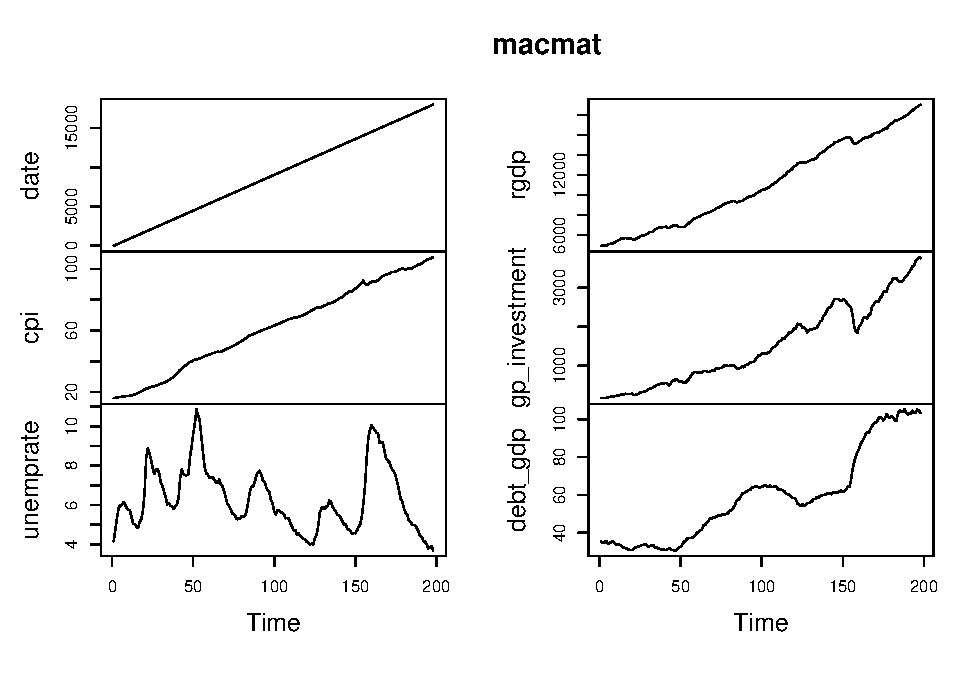
\includegraphics{solution_exercise_5_files/figure-latex/unnamed-chunk-3-1.pdf}

Every series except unemployment looks non-stationary. Regarding the
debt-to-gdp ratio, this is surprising, but we better difference it as
well.

\begin{Shaded}
\begin{Highlighting}[]
\NormalTok{macdata <-}\StringTok{ }\KeywordTok{cbind}\NormalTok{(}\KeywordTok{diff}\NormalTok{(}\KeywordTok{log}\NormalTok{(us.macro_series}\OperatorTok{$}\NormalTok{cpi)), }
\NormalTok{                 us.macro_series}\OperatorTok{$}\NormalTok{unemprate[}\OperatorTok{-}\NormalTok{(}\KeywordTok{nrow}\NormalTok{(macmat))], }
                 \KeywordTok{diff}\NormalTok{(}\KeywordTok{log}\NormalTok{(us.macro_series}\OperatorTok{$}\NormalTok{rgdp)),}
                 \KeywordTok{diff}\NormalTok{(}\KeywordTok{log}\NormalTok{(us.macro_series}\OperatorTok{$}\NormalTok{gp_investment)), }
                 \KeywordTok{diff}\NormalTok{(}\KeywordTok{log}\NormalTok{(us.macro_series}\OperatorTok{$}\NormalTok{debt_gdp)))}

\KeywordTok{plot.ts}\NormalTok{(macdata)}
\end{Highlighting}
\end{Shaded}

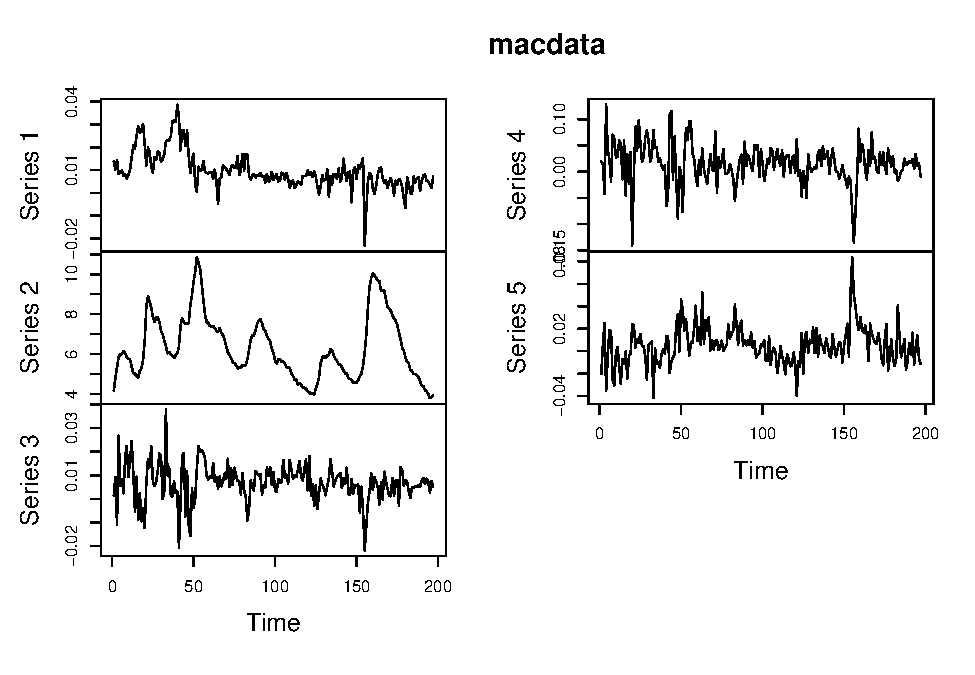
\includegraphics{solution_exercise_5_files/figure-latex/unnamed-chunk-4-1.pdf}

Note that the last observation of \enquote{unemp} was dropped for
conformable length. Its last and not first due to the date information:
measurements are always from the first day of a quarter.

\begin{itemize}
  \item[b.)] Perform a Ljung-Box test on the dataset. Does it look worthwhile to estimate a $\VAR(p)$
\end{itemize}

\emph{Solution:}

\begin{Shaded}
\begin{Highlighting}[]
\KeywordTok{mq}\NormalTok{(}\DataTypeTok{x =}\NormalTok{ macdata, }\DataTypeTok{lag =} \DecValTok{20}\NormalTok{)}
\end{Highlighting}
\end{Shaded}

\begin{verbatim}
## Ljung-Box Statistics:  
##         m       Q(m)     df    p-value
##  [1,]     1       369      25        0
##  [2,]     2       658      50        0
##  [3,]     3       932      75        0
##  [4,]     4      1211     100        0
##  [5,]     5      1430     125        0
##  [6,]     6      1624     150        0
##  [7,]     7      1796     175        0
##  [8,]     8      1953     200        0
##  [9,]     9      2083     225        0
## [10,]    10      2205     250        0
## [11,]    11      2313     275        0
## [12,]    12      2418     300        0
## [13,]    13      2513     325        0
## [14,]    14      2619     350        0
## [15,]    15      2702     375        0
## [16,]    16      2793     400        0
## [17,]    17      2881     425        0
## [18,]    18      2965     450        0
## [19,]    19      3031     475        0
## [20,]    20      3112     500        0
\end{verbatim}

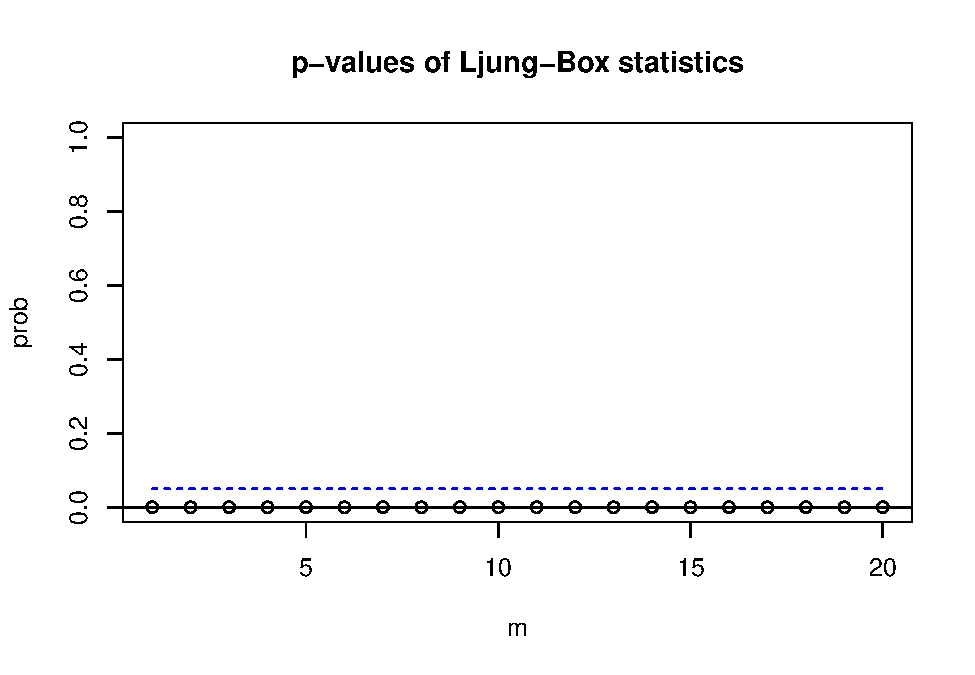
\includegraphics{solution_exercise_5_files/figure-latex/unnamed-chunk-5-1.pdf}

There is some correlation in the dataset.

\begin{Shaded}
\begin{Highlighting}[]
\KeywordTok{mq}\NormalTok{(}\DataTypeTok{x =}\NormalTok{ macdata[,}\OperatorTok{-}\DecValTok{3}\NormalTok{], }\DataTypeTok{lag =} \DecValTok{20}\NormalTok{)}
\end{Highlighting}
\end{Shaded}

\begin{verbatim}
## Ljung-Box Statistics:  
##         m       Q(m)     df    p-value
##  [1,]     1       337      16        0
##  [2,]     2       607      32        0
##  [3,]     3       866      48        0
##  [4,]     4      1121      64        0
##  [5,]     5      1325      80        0
##  [6,]     6      1502      96        0
##  [7,]     7      1650     112        0
##  [8,]     8      1781     128        0
##  [9,]     9      1894     144        0
## [10,]    10      2003     160        0
## [11,]    11      2101     176        0
## [12,]    12      2197     192        0
## [13,]    13      2278     208        0
## [14,]    14      2372     224        0
## [15,]    15      2444     240        0
## [16,]    16      2518     256        0
## [17,]    17      2589     272        0
## [18,]    18      2651     288        0
## [19,]    19      2702     304        0
## [20,]    20      2761     320        0
\end{verbatim}

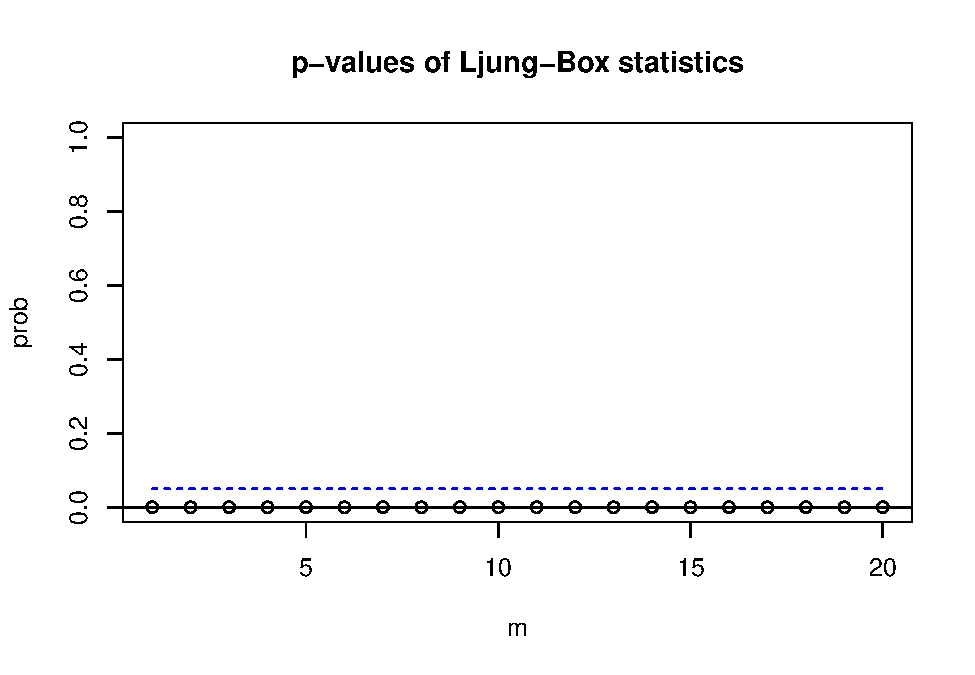
\includegraphics{solution_exercise_5_files/figure-latex/unnamed-chunk-6-1.pdf}

Even without unemployment, there is some correlation in the dataset.

\begin{itemize}
  \item[c.)] Determine the length of the time series. How many coefficients can be estimated and what does it mean for $K$ and $p$?
\end{itemize}

\emph{Solution:}

We have \(T \cdot K\) data points and we estimate \(K^2\) parameters for
each lag. For the intercept we estimate \(K\) parameters. Which leads to
the following condition for the maximal number of lag(s) \(p\):

\[ \dfrac{K \cdot (T -1)}{K^2} \geq p\]

\begin{Shaded}
\begin{Highlighting}[]
\NormalTok{data_dim <-}\StringTok{ }\KeywordTok{dim}\NormalTok{(macdata) }

\NormalTok{Tmax <-}\StringTok{ }\NormalTok{data_dim[}\DecValTok{1}\NormalTok{] }\CommentTok{# observations}
\NormalTok{K <-}\StringTok{ }\NormalTok{data_dim[}\DecValTok{2}\NormalTok{] }\CommentTok{# variables}
\NormalTok{(max.p <-}\StringTok{ }\NormalTok{(Tmax }\OperatorTok{*}\StringTok{ }\NormalTok{K }\OperatorTok{-}\StringTok{ }\NormalTok{K) }\OperatorTok{/}\StringTok{ }\NormalTok{K}\OperatorTok{^}\DecValTok{2}\NormalTok{ )}
\end{Highlighting}
\end{Shaded}

\begin{verbatim}
## [1] 39.2
\end{verbatim}

39 lags can be estimated in addition to the intercept.

\begin{itemize}
  \item[d.)] Consult the AIC, BIC and HQ to determine the optimal lag order for a $\VAR(p)$ model for the whole dataset. Plot the values of the three criteria for the lag orders p from 1 to 5 in one plot.
\end{itemize}

\emph{Solution:}

\begin{Shaded}
\begin{Highlighting}[]
\NormalTok{M <-}\StringTok{ }\DecValTok{10} \CommentTok{# maximal p }
\KeywordTok{VARorder}\NormalTok{(}\DataTypeTok{x =}\NormalTok{ macdata, }\DataTypeTok{maxp =}\NormalTok{ M)}
\end{Highlighting}
\end{Shaded}

\begin{verbatim}
## selected order: aic =  4 
## selected order: bic =  1 
## selected order: hq =  2 
## Summary table:  
##        p      AIC      BIC       HQ     M(p) p-value
##  [1,]  0 -34.8741 -34.8741 -34.8741   0.0000  0.0000
##  [2,]  1 -40.1273 -39.7107 -39.9587 994.0213  0.0000
##  [3,]  2 -40.4982 -39.6649 -40.1608 109.6255  0.0000
##  [4,]  3 -40.6510 -39.4011 -40.1450  69.3340  0.0000
##  [5,]  4 -40.7551 -39.0885 -40.0805  59.2354  0.0001
##  [6,]  5 -40.6962 -38.6129 -39.8529  31.2764  0.1800
##  [7,]  6 -40.5110 -38.0111 -39.4990  10.6681  0.9944
##  [8,]  7 -40.5487 -37.6321 -39.3680  43.8714  0.0112
##  [9,]  8 -40.5490 -37.2158 -39.1997  36.9772  0.0580
## [10,]  9 -40.4934 -36.7436 -38.9754  27.8481  0.3149
## [11,] 10 -40.4553 -36.2888 -38.7687  29.2269  0.2545
\end{verbatim}

\begin{Shaded}
\begin{Highlighting}[]
\CommentTok{# so it's p = 1, 2 or 4.....}
\NormalTok{var1to5.fit <-}\StringTok{ }\KeywordTok{lapply}\NormalTok{(}\DataTypeTok{X =} \DecValTok{1}\OperatorTok{:}\NormalTok{M, }\ControlFlowTok{function}\NormalTok{(i)}
  \KeywordTok{VAR}\NormalTok{(}\DataTypeTok{x =}\NormalTok{ macdata, }\DataTypeTok{include.mean =} \OtherTok{TRUE}\NormalTok{, }\DataTypeTok{p =}\NormalTok{ i, }\DataTypeTok{output =} \OtherTok{FALSE}\NormalTok{))}
\NormalTok{var1to5.aic <-}\StringTok{ }\KeywordTok{sapply}\NormalTok{(}\DecValTok{1}\OperatorTok{:}\NormalTok{M, }\ControlFlowTok{function}\NormalTok{(i) var1to5.fit[[i]]}\OperatorTok{$}\NormalTok{aic)}
\NormalTok{var1to5.bic <-}\StringTok{ }\KeywordTok{sapply}\NormalTok{(}\DecValTok{1}\OperatorTok{:}\NormalTok{M, }\ControlFlowTok{function}\NormalTok{(i) var1to5.fit[[i]]}\OperatorTok{$}\NormalTok{bic)}
\NormalTok{var1to5.hq <-}\StringTok{ }\KeywordTok{sapply}\NormalTok{(}\DecValTok{1}\OperatorTok{:}\NormalTok{M, }\ControlFlowTok{function}\NormalTok{(i) var1to5.fit[[i]]}\OperatorTok{$}\NormalTok{hq)}
\KeywordTok{plot}\NormalTok{(}\DataTypeTok{x =} \DecValTok{1}\OperatorTok{:}\NormalTok{M, }\DataTypeTok{y =}\NormalTok{ var1to5.aic, }\DataTypeTok{type =} \StringTok{"b"}\NormalTok{,}
     \DataTypeTok{main =} \StringTok{"Values of Information Criteria"}\NormalTok{, }\DataTypeTok{xlab =} \StringTok{"p"}\NormalTok{,}
     \DataTypeTok{ylim =} \KeywordTok{c}\NormalTok{( }\KeywordTok{min}\NormalTok{(}\KeywordTok{c}\NormalTok{(var1to5.aic, var1to5.bic, var1to5.hq)), }
               \KeywordTok{max}\NormalTok{(}\KeywordTok{c}\NormalTok{(var1to5.aic, var1to5.bic, var1to5.hq)) ) )}

\KeywordTok{points}\NormalTok{(}\DataTypeTok{x =} \DecValTok{1}\OperatorTok{:}\NormalTok{M, }\DataTypeTok{y =}\NormalTok{ var1to5.bic, }\DataTypeTok{pch =} \DecValTok{11}\NormalTok{, }\DataTypeTok{col =} \StringTok{"red"}\NormalTok{)}
\KeywordTok{points}\NormalTok{(}\DataTypeTok{x =} \DecValTok{1}\OperatorTok{:}\NormalTok{M, }\DataTypeTok{y =}\NormalTok{ var1to5.hq, }\DataTypeTok{col =} \StringTok{"blue"}\NormalTok{, }\DataTypeTok{pch =} \DecValTok{25}\NormalTok{)}
\KeywordTok{legend}\NormalTok{(}\StringTok{"topleft"}\NormalTok{, }\DataTypeTok{legend =} \KeywordTok{c}\NormalTok{(}\StringTok{"AIC"}\NormalTok{, }\StringTok{"BIC"}\NormalTok{, }\StringTok{"HQ"}\NormalTok{), }
       \DataTypeTok{col =} \KeywordTok{c}\NormalTok{(}\StringTok{"black"}\NormalTok{, }\StringTok{"red"}\NormalTok{, }\StringTok{"blue"}\NormalTok{), }
       \DataTypeTok{pch =} \KeywordTok{c}\NormalTok{(}\OtherTok{NA}\NormalTok{, }\DecValTok{11}\NormalTok{, }\DecValTok{25}\NormalTok{), }\DataTypeTok{lwd =} \KeywordTok{c}\NormalTok{(}\DecValTok{2}\NormalTok{, }\OtherTok{NA}\NormalTok{, }\OtherTok{NA}\NormalTok{))}
\end{Highlighting}
\end{Shaded}

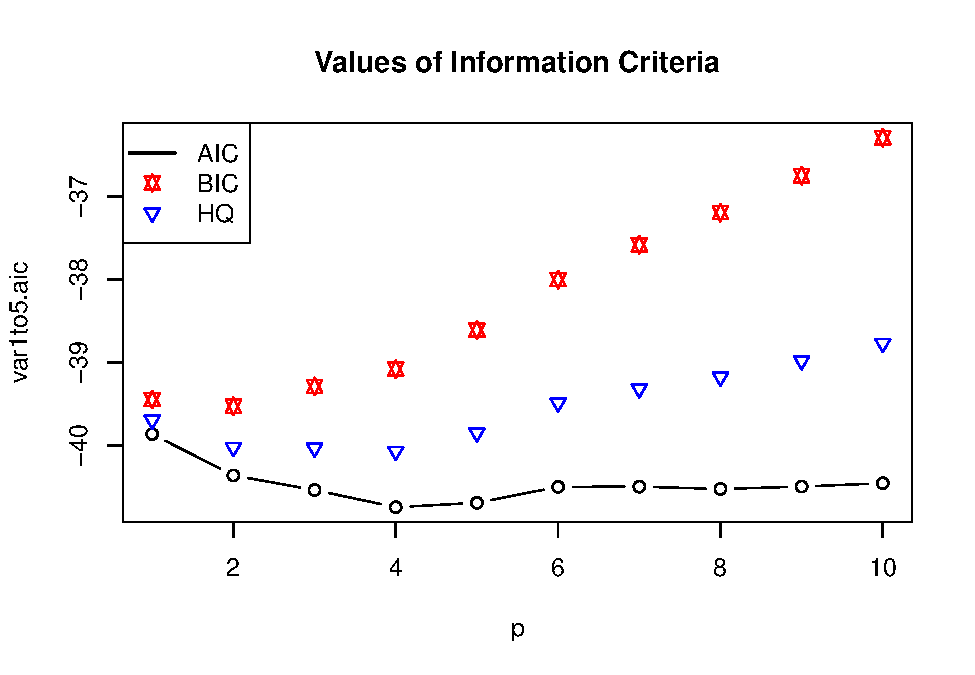
\includegraphics{solution_exercise_5_files/figure-latex/unnamed-chunk-8-1.pdf}

\begin{itemize}
  \item AIC and HQ are flat around the minima $\Rightarrow$ no distinct optimum visible. 
  \item Conceivable reasons: persistence, omitted variables,  wrong functional form
  \item The $\VAR$ may just work as an approximation
  \item BIC is the most conservative IC
  \item Mimima at:
\end{itemize}

\begin{align*}
p = 
  \begin{cases}
  1 & BIC \\
  2 & HQ \\
  4 & AIC
  \end{cases}
\end{align*}

\begin{itemize}
  \item[e.)] Fit $\VAR(p)$ models incorporating all variables using the optimal lag order(s) p suggested by each of the information criteria. Apply the Ljung-Box test to inspect the residuals’ properties. For which models does the test reject the null hypothesis on one of the first ten lags?
\end{itemize}

\emph{Solution:}

First we need to estimated a \(\VAR(p)\).

\begin{Shaded}
\begin{Highlighting}[]
\NormalTok{var1.fit <-}\StringTok{ }\KeywordTok{VAR}\NormalTok{(}\DataTypeTok{x =}\NormalTok{ macdata, }\DataTypeTok{p =} \DecValTok{1}\NormalTok{, }\DataTypeTok{include.mean =} \OtherTok{TRUE}\NormalTok{, }\DataTypeTok{output =} \OtherTok{FALSE}\NormalTok{)}
\NormalTok{var2.fit <-}\StringTok{ }\KeywordTok{VAR}\NormalTok{(}\DataTypeTok{x =}\NormalTok{ macdata, }\DataTypeTok{p =} \DecValTok{2}\NormalTok{, }\DataTypeTok{include.mean =} \OtherTok{TRUE}\NormalTok{, }\DataTypeTok{output =} \OtherTok{FALSE}\NormalTok{)}
\NormalTok{var4.fit <-}\StringTok{ }\KeywordTok{VAR}\NormalTok{(}\DataTypeTok{x =}\NormalTok{ macdata, }\DataTypeTok{p =} \DecValTok{4}\NormalTok{, }\DataTypeTok{include.mean =} \OtherTok{TRUE}\NormalTok{, }\DataTypeTok{output =} \OtherTok{FALSE}\NormalTok{)}
\end{Highlighting}
\end{Shaded}

Now the Ljung-Box test can be performed. We adjust using \(K = 5\) with
\(5^2 \times p\) degree of freedom. Adjustment for the intercept is not
necessary, since \(z_t\) needs to be demeaned anyway
\(\left(\Gamma_0 = \left(z_t - \mu \right) \left( z_t - \mu \right)^{'} \right)\).
The Ljun-Box test has \(m \times K^2\) degree of freedom (\(K^2\) per
lagged cross-correlation matrices), so after adjustment, we have
\((m - p) K^2\) degrees of freedom.

\begin{Shaded}
\begin{Highlighting}[]
\KeywordTok{mq}\NormalTok{(}\DataTypeTok{x =}\NormalTok{ var1.fit}\OperatorTok{$}\NormalTok{residuals, }\DataTypeTok{lag =} \DecValTok{25}\NormalTok{, }\DataTypeTok{adj =} \DecValTok{25} \OperatorTok{*}\StringTok{ }\DecValTok{1}\NormalTok{)}
\end{Highlighting}
\end{Shaded}

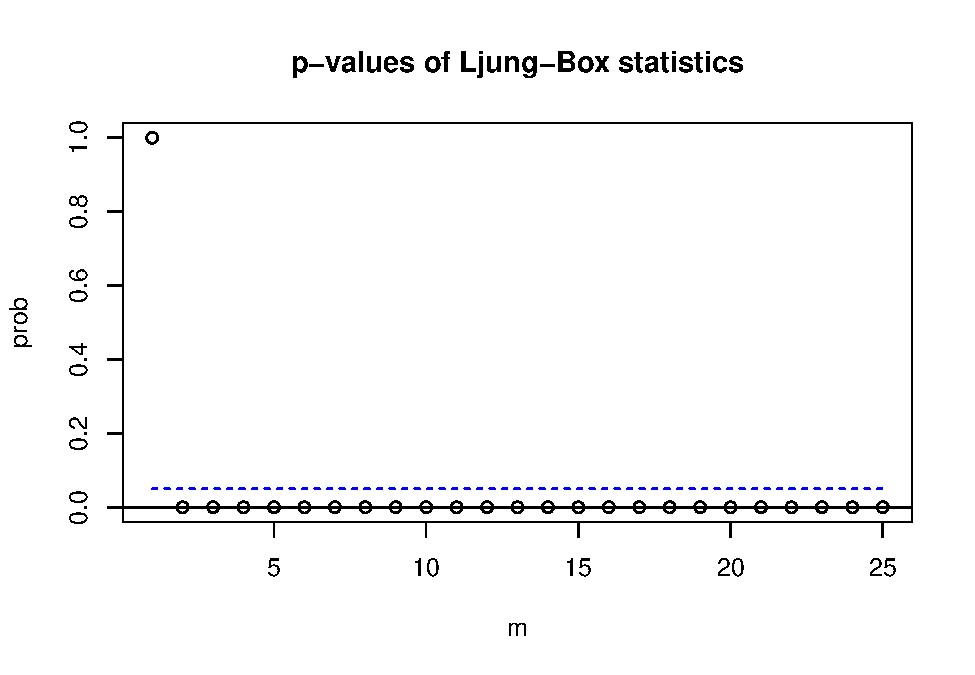
\includegraphics{solution_exercise_5_files/figure-latex/unnamed-chunk-10-1.pdf}

\begin{Shaded}
\begin{Highlighting}[]
\KeywordTok{mq}\NormalTok{(}\DataTypeTok{x =}\NormalTok{ var2.fit}\OperatorTok{$}\NormalTok{residuals, }\DataTypeTok{lag =} \DecValTok{25}\NormalTok{, }\DataTypeTok{adj =} \DecValTok{25} \OperatorTok{*}\StringTok{ }\DecValTok{2}\NormalTok{)}
\end{Highlighting}
\end{Shaded}

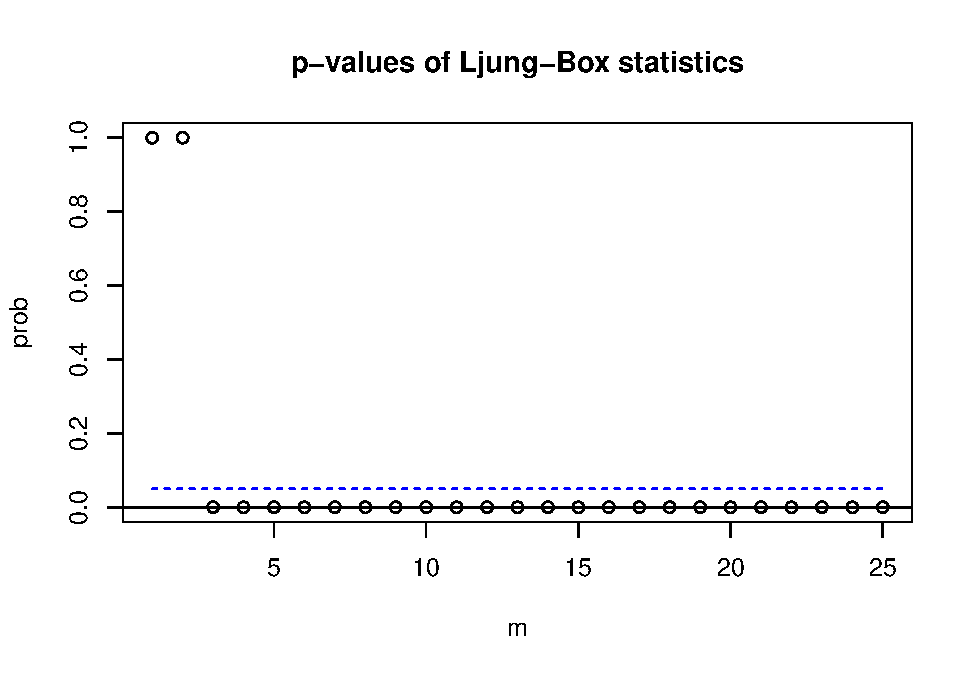
\includegraphics{solution_exercise_5_files/figure-latex/unnamed-chunk-10-2.pdf}

\begin{Shaded}
\begin{Highlighting}[]
\KeywordTok{mq}\NormalTok{(}\DataTypeTok{x =}\NormalTok{ var4.fit}\OperatorTok{$}\NormalTok{residuals, }\DataTypeTok{lag =} \DecValTok{25}\NormalTok{, }\DataTypeTok{adj =} \DecValTok{25} \OperatorTok{*}\StringTok{ }\DecValTok{4}\NormalTok{)}
\end{Highlighting}
\end{Shaded}

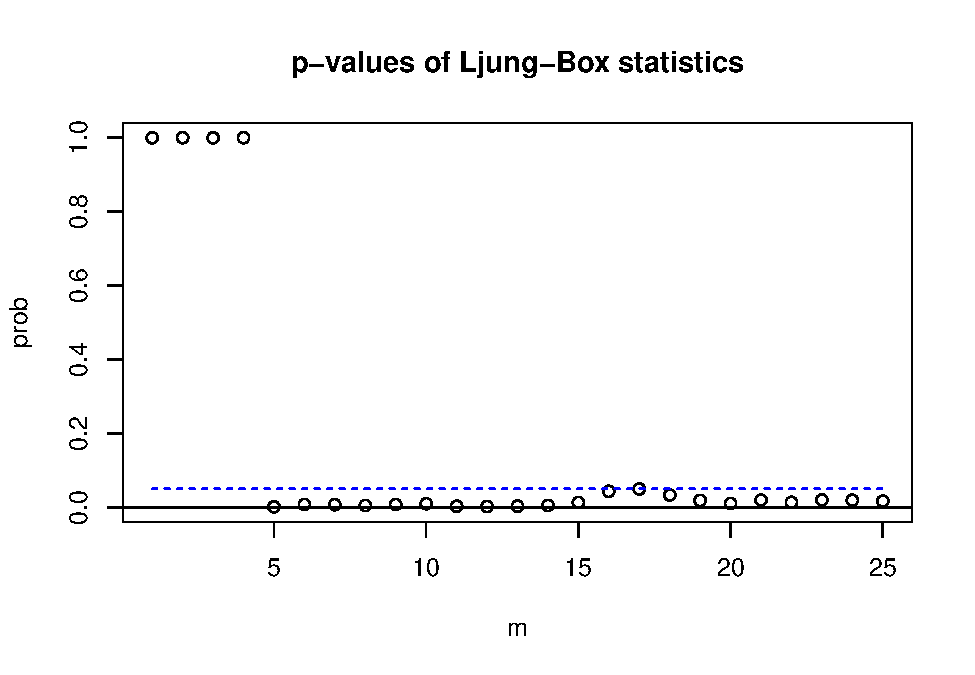
\includegraphics{solution_exercise_5_files/figure-latex/unnamed-chunk-10-3.pdf}

\begin{verbatim}
## Ljung-Box Statistics:  
##         m       Q(m)     df    p-value
##  [1,]   1.0      59.7     0.0        1
##  [2,]   2.0     113.3    25.0        0
##  [3,]   3.0     173.6    50.0        0
##  [4,]   4.0     232.8    75.0        0
##  [5,]   5.0     266.1   100.0        0
##  [6,]   6.0     298.1   125.0        0
##  [7,]   7.0     332.9   150.0        0
##  [8,]   8.0     367.1   175.0        0
##  [9,]   9.0     397.3   200.0        0
## [10,]  10.0     450.3   225.0        0
## [11,]  11.0     470.5   250.0        0
## [12,]  12.0     508.8   275.0        0
## [13,]  13.0     535.2   300.0        0
## [14,]  14.0     573.0   325.0        0
## [15,]  15.0     588.0   350.0        0
## [16,]  16.0     612.2   375.0        0
## [17,]  17.0     646.3   400.0        0
## [18,]  18.0     672.2   425.0        0
## [19,]  19.0     697.7   450.0        0
## [20,]  20.0     740.1   475.0        0
## [21,]  21.0     762.6   500.0        0
## [22,]  22.0     796.2   525.0        0
## [23,]  23.0     818.7   550.0        0
## [24,]  24.0     847.9   575.0        0
## [25,]  25.0     865.4   600.0        0
## Ljung-Box Statistics:  
##         m       Q(m)     df    p-value
##  [1,]   1.0      12.7   -25.0        1
##  [2,]   2.0      38.9     0.0        1
##  [3,]   3.0      74.3    25.0        0
##  [4,]   4.0     118.2    50.0        0
##  [5,]   5.0     151.2    75.0        0
##  [6,]   6.0     173.3   100.0        0
##  [7,]   7.0     208.2   125.0        0
##  [8,]   8.0     251.8   150.0        0
##  [9,]   9.0     282.7   175.0        0
## [10,]  10.0     320.9   200.0        0
## [11,]  11.0     346.2   225.0        0
## [12,]  12.0     385.0   250.0        0
## [13,]  13.0     407.7   275.0        0
## [14,]  14.0     444.4   300.0        0
## [15,]  15.0     460.8   325.0        0
## [16,]  16.0     481.2   350.0        0
## [17,]  17.0     511.5   375.0        0
## [18,]  18.0     536.5   400.0        0
## [19,]  19.0     564.8   425.0        0
## [20,]  20.0     600.8   450.0        0
## [21,]  21.0     626.8   475.0        0
## [22,]  22.0     659.7   500.0        0
## [23,]  23.0     686.5   525.0        0
## [24,]  24.0     721.5   550.0        0
## [25,]  25.0     742.9   575.0        0
## Ljung-Box Statistics:  
##          m       Q(m)     df    p-value
##  [1,]   1.00      3.38  -75.00     1.00
##  [2,]   2.00     10.06  -50.00     1.00
##  [3,]   3.00     17.79  -25.00     1.00
##  [4,]   4.00     31.52    0.00     1.00
##  [5,]   5.00     52.36   25.00     0.00
##  [6,]   6.00     77.69   50.00     0.01
##  [7,]   7.00    108.50   75.00     0.01
##  [8,]   8.00    140.58  100.00     0.00
##  [9,]   9.00    166.97  125.00     0.01
## [10,]  10.00    193.58  150.00     0.01
## [11,]  11.00    231.30  175.00     0.00
## [12,]  12.00    262.58  200.00     0.00
## [13,]  13.00    287.90  225.00     0.00
## [14,]  14.00    311.71  250.00     0.00
## [15,]  15.00    329.90  275.00     0.01
## [16,]  16.00    343.34  300.00     0.04
## [17,]  17.00    368.22  325.00     0.05
## [18,]  18.00    400.16  350.00     0.03
## [19,]  19.00    434.46  375.00     0.02
## [20,]  20.00    468.69  400.00     0.01
## [21,]  21.00    487.46  425.00     0.02
## [22,]  22.00    519.00  450.00     0.01
## [23,]  23.00    540.71  475.00     0.02
## [24,]  24.00    567.70  500.00     0.02
## [25,]  25.00    596.44  525.00     0.02
\end{verbatim}

Since the tests rejects everywhere else, the VARs do not explain the
dynamics entirely.

\begin{itemize}
  \item[f.)] Now take a $\VAR(1)$ and a $\VAR(4)$ model with all variables included and an intercept specified.
  \begin{enumerate}[label=(\roman*)]
    \item How many coefficients are estimated in each case?
    \item Look at both estimates of $\Sigma_a$ - are there major difference?
    \item Compare the standard errors associated with the $\phi_1$ matrices of the $\VAR(1)$ and $\VAR(4)$ from above. Do you see the same pattern regarding $\Sigma_a$? 
  \end{enumerate}
\end{itemize}

\emph{Solution:}

\begin{enumerate}[label=(\roman*)]
    \item How many coefficients are estimated in each case?
    
    The formula for computing the number of parameters is $K^2 \times p + K$. For a $\VAR(1)$ we estimate 30 parameters. Whereas for a $\VAR(4)$ we already need to estimate  105 parameters. 
    
    \item Look at both estimates of $\Sigma_a$ - are there major difference?

    Ratio of residual coveriances: 
  \end{enumerate}

\begin{Shaded}
\begin{Highlighting}[]
\NormalTok{var1.fit}\OperatorTok{$}\NormalTok{Sigma }\OperatorTok{/}\StringTok{ }\NormalTok{var4.fit}\OperatorTok{$}\NormalTok{Sigma}
\end{Highlighting}
\end{Shaded}

\begin{verbatim}
##           [,1]      [,2]     [,3]     [,4]     [,5]
## [1,] 1.2908794 0.7594541 1.179527 1.161651 1.115374
## [2,] 0.7594541 1.8963595 1.535077 1.242121 1.946967
## [3,] 1.1795272 1.5350769 1.216217 1.282319 1.276541
## [4,] 1.1616514 1.2421212 1.282319 1.272154 1.256466
## [5,] 1.1153745 1.9469672 1.276541 1.256466 1.291657
\end{verbatim}

Reisdual (co)variances are higher for the \(\VAR(1)\). \(\VAR(4)\)
predicts better (in-sample).

\begin{enumerate}[label=(\roman*)]
    \setcounter{enumi}{2}
    \item Compare the standard errors associated with the $\phi_1$ matrices of the $\VAR(1)$ and $\VAR(4)$ from above. Do you see the same pattern regarding $\Sigma_a$? 
  \end{enumerate}

Ratio of standard errors:

\begin{Shaded}
\begin{Highlighting}[]
\NormalTok{var1.fit}\OperatorTok{$}\NormalTok{secoef }\OperatorTok{/}\StringTok{ }\NormalTok{var4.fit}\OperatorTok{$}\NormalTok{secoef[}\DecValTok{1}\OperatorTok{:}\DecValTok{6}\NormalTok{,]}
\end{Highlighting}
\end{Shaded}

\begin{verbatim}
##           [,1]      [,2]      [,3]      [,4]      [,5]
## [1,] 0.7270512 0.8812163 0.7057122 0.7217587 0.7272702
## [2,] 0.6486366 0.7861744 0.6295990 0.6439149 0.6488319
## [3,] 0.1268594 0.1537589 0.1231361 0.1259359 0.1268976
## [4,] 0.9832151 1.1916975 0.9543577 0.9760579 0.9835113
## [5,] 0.9100956 1.1030737 0.8833843 0.9034707 0.9103698
## [6,] 0.9956293 1.2067440 0.9664075 0.9883817 0.9959292
\end{verbatim}

No, it is exactly the other way around. Estimating more coefficients
with the same information leads to less information per coefficient.

\begin{itemize}
  \item[g.)]  Repeat the task from above with CPI and the debt-to-gdp ratio as the only variables (hence $K = 2$). How many coefficients are estimated in this case?
\end{itemize}

With only two explanatory variables we can estimated maximally 98 lags.

\begin{Shaded}
\begin{Highlighting}[]
\NormalTok{var1red.fit <-}\StringTok{ }\KeywordTok{VAR}\NormalTok{(}\DataTypeTok{x =}\NormalTok{ macdata[,}\KeywordTok{c}\NormalTok{(}\DecValTok{1}\NormalTok{,}\DecValTok{5}\NormalTok{)], }\DataTypeTok{p =} \DecValTok{1}\NormalTok{, }\DataTypeTok{output =} \OtherTok{FALSE}\NormalTok{, }\DataTypeTok{include.mean =} \OtherTok{TRUE}\NormalTok{)}
\NormalTok{var4red.fit <-}\StringTok{ }\KeywordTok{VAR}\NormalTok{(}\DataTypeTok{x =}\NormalTok{ macdata[,}\KeywordTok{c}\NormalTok{(}\DecValTok{1}\NormalTok{,}\DecValTok{5}\NormalTok{)], }\DataTypeTok{p =} \DecValTok{4}\NormalTok{, }\DataTypeTok{output =} \OtherTok{FALSE}\NormalTok{, }\DataTypeTok{include.mean =} \OtherTok{TRUE}\NormalTok{)}
\end{Highlighting}
\end{Shaded}

For a \(\VAR(1)\) 6 coefficients are estimated, for a \(\VAR(4)\) 18
coefficients.

Any major differences between the residual covariance matrices?

Ratio of residual coveriances:

\begin{Shaded}
\begin{Highlighting}[]
\NormalTok{var1red.fit}\OperatorTok{$}\NormalTok{Sigma }\OperatorTok{/}\StringTok{ }\NormalTok{var4red.fit}\OperatorTok{$}\NormalTok{Sigma}
\end{Highlighting}
\end{Shaded}

\begin{verbatim}
##           [,1]      [,2]
## [1,] 1.1763704 0.9715465
## [2,] 0.9715465 1.2602521
\end{verbatim}

Ratio of standard errors:

\begin{Shaded}
\begin{Highlighting}[]
\NormalTok{var1red.fit}\OperatorTok{$}\NormalTok{secoef }\OperatorTok{/}\StringTok{ }\NormalTok{var4red.fit}\OperatorTok{$}\NormalTok{secoef[}\DecValTok{1}\OperatorTok{:}\DecValTok{3}\NormalTok{,]}
\end{Highlighting}
\end{Shaded}

\begin{verbatim}
##           [,1]      [,2]
## [1,] 0.9299869 0.9625727
## [2,] 0.6319156 0.6540572
## [3,] 0.9201816 0.9524238
\end{verbatim}

\begin{itemize}
  \item[h.)] At last, go back to $\VAR(1)$ and $\VAR(4)$ models from task f). Use the standard error matrices to compute t-statistics for each coefficient with the null hypothesis $H_0: phi_(p,jk) = 0$. How often is the null hypothesis rejected at the 5\% level in each of the two models? 
\end{itemize}

To compute the t-statistic the estimated parameters get divided by the
standard error of the parameter.

\begin{Shaded}
\begin{Highlighting}[]
\NormalTok{var1.t_ratios <-}\StringTok{ }\NormalTok{var1.fit}\OperatorTok{$}\NormalTok{coef }\OperatorTok{/}\StringTok{ }\NormalTok{var1.fit}\OperatorTok{$}\NormalTok{secoef}
\NormalTok{var2.t_ratios <-}\StringTok{ }\NormalTok{var2.fit}\OperatorTok{$}\NormalTok{coef }\OperatorTok{/}\StringTok{ }\NormalTok{var2.fit}\OperatorTok{$}\NormalTok{secoef}
\NormalTok{var4.t_ratios <-}\StringTok{ }\NormalTok{var4.fit}\OperatorTok{$}\NormalTok{coef }\OperatorTok{/}\StringTok{ }\NormalTok{var4.fit}\OperatorTok{$}\NormalTok{secoef}
\end{Highlighting}
\end{Shaded}

To test how often the \(H_0\) is rejected we just count how often the
t-value is absolute greater than 1.96
(\texttt{sum(abs(var1.t\_ratios\ )\ \textgreater{}\ 1.96)}). For the
\(\VAR(1)\) the \(H_0\) is 16 times which are 0.5333 of all parameters.
For a \(\VAR(2)\) 21 times the null hypothesis is rejected (0.3818) and
for a \(\VAR(4)\) 22 times (0.2095).

Same pattern as in f), but not that pronounced this time.

\hypertarget{exercise-3-this-exercise-is-concerned-with-predicting-growth-rates-of-exchange-rates.-please-download-the-file-quandl_fx_download.r-from-the-moodle-and-install-the-package-quandl.-executing-the-script-will-then-download-and-prepare-the-two-time-series-we-are-interested-in.}{%
\section{\texorpdfstring{Exercise 3: This exercise is concerned with
predicting growth rates of \n exchange rates. Please download the file
\texttt{quandl\_fx\_download.R} from the Moodle and install the package
\texttt{Quandl}. Executing the script will then download and prepare the
two time series we are interested
in.}{Exercise 3: This exercise is concerned with predicting growth rates of exchange rates. Please download the file quandl\_fx\_download.R from the Moodle and install the package Quandl. Executing the script will then download and prepare the two time series we are interested in.}}\label{exercise-3-this-exercise-is-concerned-with-predicting-growth-rates-of-exchange-rates.-please-download-the-file-quandl_fx_download.r-from-the-moodle-and-install-the-package-quandl.-executing-the-script-will-then-download-and-prepare-the-two-time-series-we-are-interested-in.}}

To download the data from \texttt{Quandl} you need your own API key and
execture the following code.

\begin{Shaded}
\begin{Highlighting}[]
\KeywordTok{library}\NormalTok{(Quandl)}
\CommentTok{# Set API key}
\KeywordTok{Quandl.api_key}\NormalTok{(}\StringTok{""}\NormalTok{) }\CommentTok{# Please enter your key in here.}

\CommentTok{## Download and prepare data}

\CommentTok{# Download daily data on Japan/US FX rates}
\NormalTok{FX.Ja   <-}\StringTok{ }\KeywordTok{Quandl}\NormalTok{(}\StringTok{"FRED/DEXJPUS"}\NormalTok{, }\DataTypeTok{start_date =} \StringTok{"1998-12-30"}\NormalTok{, }
                  \DataTypeTok{end_date =} \StringTok{"2018-12-31"}\NormalTok{, }\DataTypeTok{type =} \StringTok{"xts"}\NormalTok{)   }
\CommentTok{# Download daily data on Euro/US FX rates}
\NormalTok{FX.Eu   <-}\StringTok{ }\KeywordTok{Quandl}\NormalTok{(}\StringTok{"FRED/DEXUSEU"}\NormalTok{, }\DataTypeTok{start_date =} \StringTok{"1998-12-30"}\NormalTok{, }
                  \DataTypeTok{end_date =} \StringTok{"2018-12-31"}\NormalTok{, }\DataTypeTok{type =} \StringTok{"xts"}\NormalTok{)  }

\CommentTok{# Compute Growth rates}
\NormalTok{lr.Eu <-}\StringTok{ }\KeywordTok{diff}\NormalTok{(}\KeywordTok{log}\NormalTok{(FX.Eu[, }\DecValTok{1}\NormalTok{]))[}\OperatorTok{-}\DecValTok{1}\NormalTok{] }\CommentTok{# leave out NA in first component via [-1]}
\NormalTok{lr.Ja <-}\StringTok{ }\KeywordTok{diff}\NormalTok{(}\KeywordTok{log}\NormalTok{(FX.Ja[, }\DecValTok{1}\NormalTok{]))[}\OperatorTok{-}\DecValTok{1}\NormalTok{] }\CommentTok{# leave out NA in first component via [-1]}

\CommentTok{# only use data when both log-returns are available}
\NormalTok{V         <-}\StringTok{ }\KeywordTok{merge.xts}\NormalTok{(lr.Eu, lr.Ja, }\DataTypeTok{all=}\OtherTok{FALSE}\NormalTok{)  }

\NormalTok{date      <-}\StringTok{ }\KeywordTok{index}\NormalTok{(V)   }\CommentTok{# save dates for later use}
\NormalTok{fx_series <-}\StringTok{ }\KeywordTok{coredata}\NormalTok{(V)  }\CommentTok{# raw log-returns}
\NormalTok{N         <-}\StringTok{ }\KeywordTok{length}\NormalTok{(date)}
\end{Highlighting}
\end{Shaded}

\begin{itemize}
  \item[a.)] Apply the Ljung-Box test on the multivariate time series and comment. 
\end{itemize}

\begin{Shaded}
\begin{Highlighting}[]
\KeywordTok{mq}\NormalTok{(}\DataTypeTok{x =}\NormalTok{ fx_series, }\DataTypeTok{lag =} \DecValTok{35}\NormalTok{)}
\end{Highlighting}
\end{Shaded}

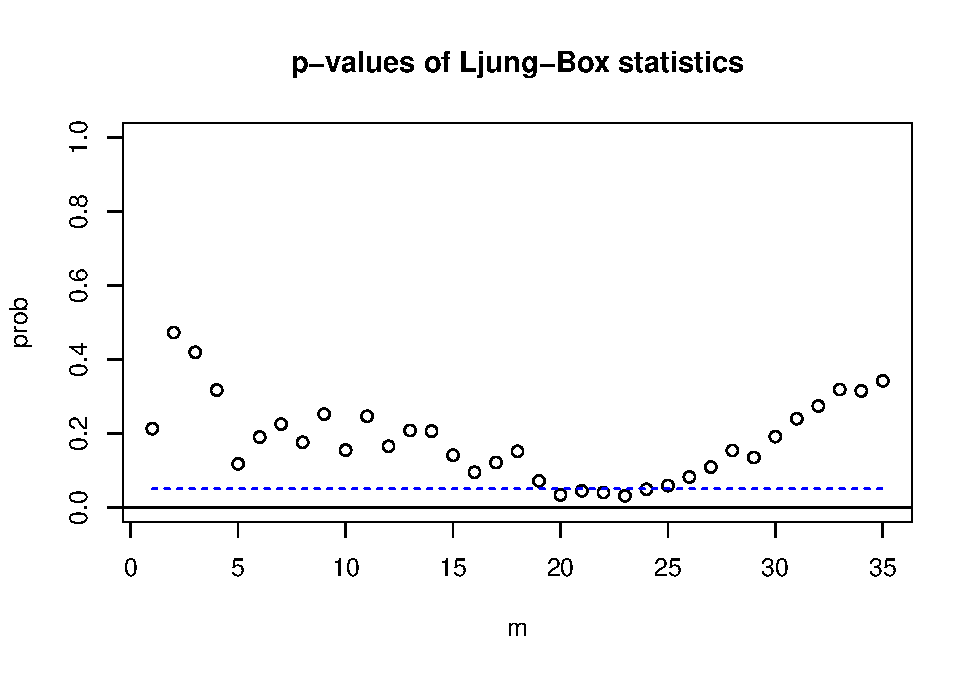
\includegraphics{solution_exercise_5_files/figure-latex/unnamed-chunk-19-1.pdf}

\begin{verbatim}
## Ljung-Box Statistics:  
##          m       Q(m)     df    p-value
##  [1,]   1.00      5.83    4.00     0.21
##  [2,]   2.00      7.61    8.00     0.47
##  [3,]   3.00     12.33   12.00     0.42
##  [4,]   4.00     18.12   16.00     0.32
##  [5,]   5.00     27.67   20.00     0.12
##  [6,]   6.00     29.85   24.00     0.19
##  [7,]   7.00     33.30   28.00     0.22
##  [8,]   8.00     39.29   32.00     0.18
##  [9,]   9.00     41.25   36.00     0.25
## [10,]  10.00     49.05   40.00     0.15
## [11,]  11.00     50.04   44.00     0.25
## [12,]  12.00     57.44   48.00     0.17
## [13,]  13.00     60.02   52.00     0.21
## [14,]  14.00     64.41   56.00     0.21
## [15,]  15.00     71.85   60.00     0.14
## [16,]  16.00     79.25   64.00     0.09
## [17,]  17.00     81.83   68.00     0.12
## [18,]  18.00     84.36   72.00     0.15
## [19,]  19.00     94.80   76.00     0.07
## [20,]  20.00    104.72   80.00     0.03
## [21,]  21.00    107.29   84.00     0.04
## [22,]  22.00    112.58   88.00     0.04
## [23,]  23.00    118.91   92.00     0.03
## [24,]  24.00    120.12   96.00     0.05
## [25,]  25.00    123.08  100.00     0.06
## [26,]  26.00    124.67  104.00     0.08
## [27,]  27.00    126.42  108.00     0.11
## [28,]  28.00    127.27  112.00     0.15
## [29,]  29.00    132.94  116.00     0.13
## [30,]  30.00    133.34  120.00     0.19
## [31,]  31.00    134.78  124.00     0.24
## [32,]  32.00    137.16  128.00     0.27
## [33,]  33.00    139.13  132.00     0.32
## [34,]  34.00    143.42  136.00     0.31
## [35,]  35.00    146.23  140.00     0.34
\end{verbatim}

Except those correlations around lag \(20\) to \(24\), there seems to be
no commanding dynamic pattern here.

\begin{itemize}
  \item[b.)] Do the usual information criteria support the finding of the Ljung-Box test? 
\end{itemize}

\begin{Shaded}
\begin{Highlighting}[]
\KeywordTok{VARorder}\NormalTok{(}\DataTypeTok{x =}\NormalTok{ fx_series, }\DataTypeTok{maxp =} \DecValTok{35}\NormalTok{)}
\end{Highlighting}
\end{Shaded}

\begin{verbatim}
## selected order: aic =  0 
## selected order: bic =  0 
## selected order: hq =  0 
## Summary table:  
##        p      AIC      BIC       HQ    M(p) p-value
##  [1,]  0 -20.3509 -20.3509 -20.3509  0.0000  0.0000
##  [2,]  1 -20.3504 -20.3452 -20.3485  5.0619  0.2810
##  [3,]  2 -20.3493 -20.3389 -20.3456  2.5648  0.6331
##  [4,]  3 -20.3484 -20.3328 -20.3429  3.4809  0.4808
##  [5,]  4 -20.3480 -20.3272 -20.3407  5.8327  0.2120
##  [6,]  5 -20.3485 -20.3226 -20.3394 10.6929  0.0302
##  [7,]  6 -20.3474 -20.3162 -20.3364  2.0955  0.7182
##  [8,]  7 -20.3463 -20.3100 -20.3336  2.8209  0.5882
##  [9,]  8 -20.3460 -20.3045 -20.3315  6.5108  0.1641
## [10,]  9 -20.3448 -20.2980 -20.3284  1.6483  0.8001
## [11,] 10 -20.3447 -20.2928 -20.3265  7.5959  0.1076
## [12,] 11 -20.3433 -20.2862 -20.3233  0.8605  0.9302
## [13,] 12 -20.3435 -20.2811 -20.3216  8.7104  0.0688
## [14,] 13 -20.3423 -20.2748 -20.3187  2.3603  0.6698
## [15,] 14 -20.3417 -20.2690 -20.3162  4.6531  0.3248
## [16,] 15 -20.3419 -20.2640 -20.3146  9.0812  0.0591
## [17,] 16 -20.3421 -20.2590 -20.3130  8.6706  0.0699
## [18,] 17 -20.3409 -20.2526 -20.3100  2.1661  0.7052
## [19,] 18 -20.3398 -20.2463 -20.3070  2.3256  0.6761
## [20,] 19 -20.3403 -20.2415 -20.3057 10.0891  0.0390
## [21,] 20 -20.3407 -20.2368 -20.3043 10.1670  0.0377
## [22,] 21 -20.3396 -20.2305 -20.3014  2.4550  0.6527
## [23,] 22 -20.3393 -20.2250 -20.2992  6.0724  0.1938
## [24,] 23 -20.3391 -20.2197 -20.2973  7.2942  0.1211
## [25,] 24 -20.3379 -20.2132 -20.2942  1.8071  0.7712
## [26,] 25 -20.3369 -20.2070 -20.2913  2.6354  0.6206
## [27,] 26 -20.3356 -20.2005 -20.2883  1.5773  0.8129
## [28,] 27 -20.3344 -20.1941 -20.2853  2.1157  0.7145
## [29,] 28 -20.3330 -20.1875 -20.2820  0.7476  0.9453
## [30,] 29 -20.3326 -20.1820 -20.2798  6.1498  0.1882
## [31,] 30 -20.3311 -20.1753 -20.2765  0.4671  0.9766
## [32,] 31 -20.3299 -20.1689 -20.2735  1.7841  0.7754
## [33,] 32 -20.3287 -20.1625 -20.2705  2.0704  0.7228
## [34,] 33 -20.3276 -20.1562 -20.2676  2.4413  0.6552
## [35,] 34 -20.3268 -20.1502 -20.2649  3.8463  0.4272
## [36,] 35 -20.3259 -20.1441 -20.2622  3.4624  0.4836
\end{verbatim}

The information criterias (AIC, BIC, and HQ) support the findings of the
Ljung-Box test.

\begin{itemize}
  \item[c.)] Regardless of a) and b), fit a $\VAR(1)$ to the time series. Compare $\Sigma_a$ with $\Gamma_0$. 
\end{itemize}

\begin{Shaded}
\begin{Highlighting}[]
\NormalTok{fx_var1.fit <-}\StringTok{ }\KeywordTok{VAR}\NormalTok{(}\DataTypeTok{x =}\NormalTok{ fx_series, }\DataTypeTok{p =} \DecValTok{1}\NormalTok{, }\DataTypeTok{include.mean =} \OtherTok{TRUE}\NormalTok{, }\DataTypeTok{output =} \OtherTok{FALSE}\NormalTok{)}
\NormalTok{( Gamma_}\DecValTok{0}\NormalTok{ <-}\StringTok{ }\KeywordTok{cov}\NormalTok{(fx_series))}
\end{Highlighting}
\end{Shaded}

\begin{verbatim}
##               lr.Eu         lr.Ja
## lr.Eu  3.807917e-05 -1.129738e-05
## lr.Ja -1.129738e-05  4.206437e-05
\end{verbatim}

\begin{Shaded}
\begin{Highlighting}[]
\NormalTok{(fx_var1.fit}\OperatorTok{$}\NormalTok{Sigma)}
\end{Highlighting}
\end{Shaded}

\begin{verbatim}
##               [,1]          [,2]
## [1,]  3.804083e-05 -1.128310e-05
## [2,] -1.128310e-05  4.202843e-05
\end{verbatim}

\begin{Shaded}
\begin{Highlighting}[]
\NormalTok{fx_var1.fit}\OperatorTok{$}\NormalTok{Sigma }\OperatorTok{/}\StringTok{ }\NormalTok{Gamma_}\DecValTok{0}
\end{Highlighting}
\end{Shaded}

\begin{verbatim}
##           lr.Eu     lr.Ja
## lr.Eu 0.9989932 0.9987354
## lr.Ja 0.9987354 0.9991455
\end{verbatim}

No important difference. here is almost no variation taken away by the
\(\VAR(1)\).

\begin{itemize}
  \item[d.)] Apply the Ljung-Box test on the residuals. Do the results surprise you? 
\end{itemize}

\begin{Shaded}
\begin{Highlighting}[]
\KeywordTok{mq}\NormalTok{(}\DataTypeTok{x =}\NormalTok{ fx_var1.fit}\OperatorTok{$}\NormalTok{residuals, }\DataTypeTok{lag =} \DecValTok{35}\NormalTok{, }\DataTypeTok{adj =} \DecValTok{2}\OperatorTok{^}\DecValTok{2} \OperatorTok{*}\StringTok{ }\DecValTok{1}\NormalTok{)}
\end{Highlighting}
\end{Shaded}

\begin{verbatim}
## Ljung-Box Statistics:  
##            m       Q(m)      df    p-value
##  [1,] 1.00e+00  3.78e-03 0.00e+00     1.00
##  [2,] 2.00e+00  1.77e+00 4.00e+00     0.78
##  [3,] 3.00e+00  6.72e+00 8.00e+00     0.57
##  [4,] 4.00e+00  1.26e+01 1.20e+01     0.40
##  [5,] 5.00e+00  2.19e+01 1.60e+01     0.15
##  [6,] 6.00e+00  2.43e+01 2.00e+01     0.23
##  [7,] 7.00e+00  2.78e+01 2.40e+01     0.27
##  [8,] 8.00e+00  3.38e+01 2.80e+01     0.21
##  [9,] 9.00e+00  3.57e+01 3.20e+01     0.30
## [10,] 1.00e+01  4.34e+01 3.60e+01     0.19
## [11,] 1.10e+01  4.42e+01 4.00e+01     0.30
## [12,] 1.20e+01  5.17e+01 4.40e+01     0.20
## [13,] 1.30e+01  5.41e+01 4.80e+01     0.25
## [14,] 1.40e+01  5.87e+01 5.20e+01     0.24
## [15,] 1.50e+01  6.65e+01 5.60e+01     0.16
## [16,] 1.60e+01  7.38e+01 6.00e+01     0.11
## [17,] 1.70e+01  7.64e+01 6.40e+01     0.14
## [18,] 1.80e+01  7.89e+01 6.80e+01     0.17
## [19,] 1.90e+01  8.90e+01 7.20e+01     0.08
## [20,] 2.00e+01  9.91e+01 7.60e+01     0.04
## [21,] 2.10e+01  1.02e+02 8.00e+01     0.05
## [22,] 2.20e+01  1.07e+02 8.40e+01     0.05
## [23,] 2.30e+01  1.13e+02 8.80e+01     0.04
## [24,] 2.40e+01  1.15e+02 9.20e+01     0.05
## [25,] 2.50e+01  1.18e+02 9.60e+01     0.06
## [26,] 2.60e+01  1.20e+02 1.00e+02     0.09
## [27,] 2.70e+01  1.21e+02 1.04e+02     0.12
## [28,] 2.80e+01  1.22e+02 1.08e+02     0.16
## [29,] 2.90e+01  1.28e+02 1.12e+02     0.15
## [30,] 3.00e+01  1.28e+02 1.16e+02     0.21
## [31,] 3.10e+01  1.30e+02 1.20e+02     0.26
## [32,] 3.20e+01  1.32e+02 1.24e+02     0.29
## [33,] 3.30e+01  1.34e+02 1.28e+02     0.34
## [34,] 3.40e+01  1.38e+02 1.32e+02     0.33
## [35,] 3.50e+01  1.41e+02 1.36e+02     0.36
\end{verbatim}

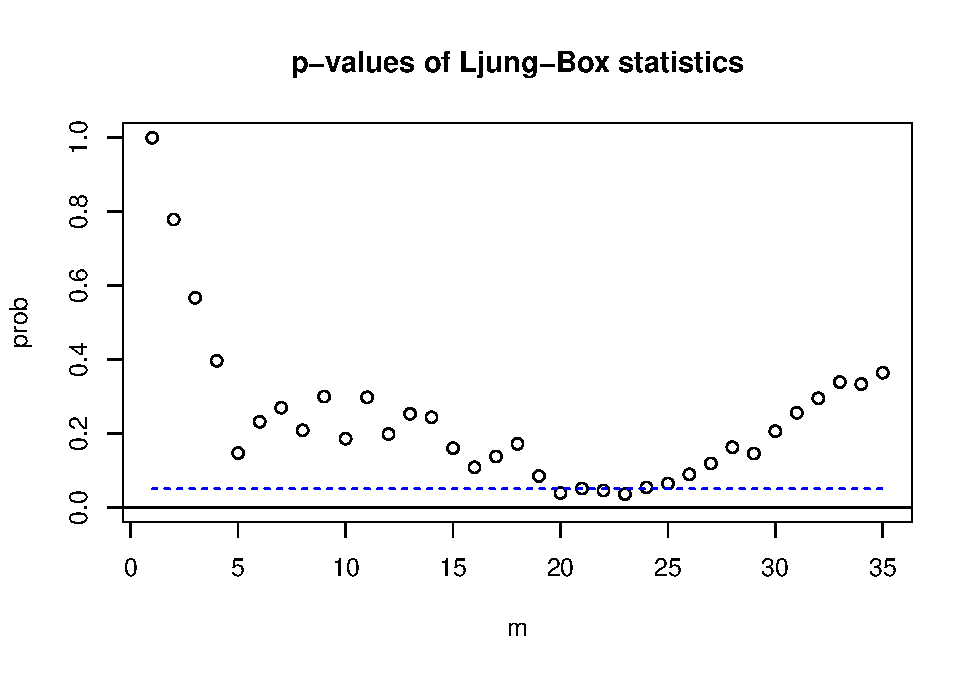
\includegraphics{solution_exercise_5_files/figure-latex/unnamed-chunk-22-1.pdf}

No.~c) has shown that nothing has changed at all.

\begin{itemize}
  \item[e.)] Repeat the Ljung-Box test but this time with the squared residuals. Also have a look at the information criteria. 
\end{itemize}

\begin{Shaded}
\begin{Highlighting}[]
\KeywordTok{mq}\NormalTok{(}\DataTypeTok{x =}\NormalTok{ fx_var1.fit}\OperatorTok{$}\NormalTok{residuals}\OperatorTok{^}\DecValTok{2}\NormalTok{, }\DataTypeTok{lag =} \DecValTok{50}\NormalTok{, }\DataTypeTok{adj =} \DecValTok{2}\OperatorTok{^}\DecValTok{2} \OperatorTok{*}\StringTok{ }\DecValTok{1}\NormalTok{)}
\end{Highlighting}
\end{Shaded}

\begin{verbatim}
## Ljung-Box Statistics:  
##          m       Q(m)     df    p-value
##  [1,]    1.0      67.4     0.0        1
##  [2,]    2.0     236.3     4.0        0
##  [3,]    3.0     272.9     8.0        0
##  [4,]    4.0     355.4    12.0        0
##  [5,]    5.0     401.8    16.0        0
##  [6,]    6.0     486.6    20.0        0
##  [7,]    7.0     546.6    24.0        0
##  [8,]    8.0     602.2    28.0        0
##  [9,]    9.0     701.2    32.0        0
## [10,]   10.0     744.7    36.0        0
## [11,]   11.0     872.9    40.0        0
## [12,]   12.0     933.1    44.0        0
## [13,]   13.0    1085.4    48.0        0
## [14,]   14.0    1130.8    52.0        0
## [15,]   15.0    1215.3    56.0        0
## [16,]   16.0    1271.8    60.0        0
## [17,]   17.0    1329.8    64.0        0
## [18,]   18.0    1384.4    68.0        0
## [19,]   19.0    1414.6    72.0        0
## [20,]   20.0    1515.5    76.0        0
## [21,]   21.0    1559.3    80.0        0
## [22,]   22.0    1665.3    84.0        0
## [23,]   23.0    1709.9    88.0        0
## [24,]   24.0    1786.0    92.0        0
## [25,]   25.0    1823.2    96.0        0
## [26,]   26.0    1864.1   100.0        0
## [27,]   27.0    1954.8   104.0        0
## [28,]   28.0    1991.2   108.0        0
## [29,]   29.0    2168.8   112.0        0
## [30,]   30.0    2197.2   116.0        0
## [31,]   31.0    2236.4   120.0        0
## [32,]   32.0    2255.5   124.0        0
## [33,]   33.0    2341.5   128.0        0
## [34,]   34.0    2379.0   132.0        0
## [35,]   35.0    2424.5   136.0        0
## [36,]   36.0    2509.7   140.0        0
## [37,]   37.0    2581.5   144.0        0
## [38,]   38.0    2640.0   148.0        0
## [39,]   39.0    2655.7   152.0        0
## [40,]   40.0    2739.5   156.0        0
## [41,]   41.0    2784.3   160.0        0
## [42,]   42.0    2825.4   164.0        0
## [43,]   43.0    2835.0   168.0        0
## [44,]   44.0    2890.5   172.0        0
## [45,]   45.0    2921.3   176.0        0
## [46,]   46.0    2949.7   180.0        0
## [47,]   47.0    3034.6   184.0        0
## [48,]   48.0    3053.4   188.0        0
## [49,]   49.0    3180.2   192.0        0
## [50,]   50.0    3219.8   196.0        0
\end{verbatim}

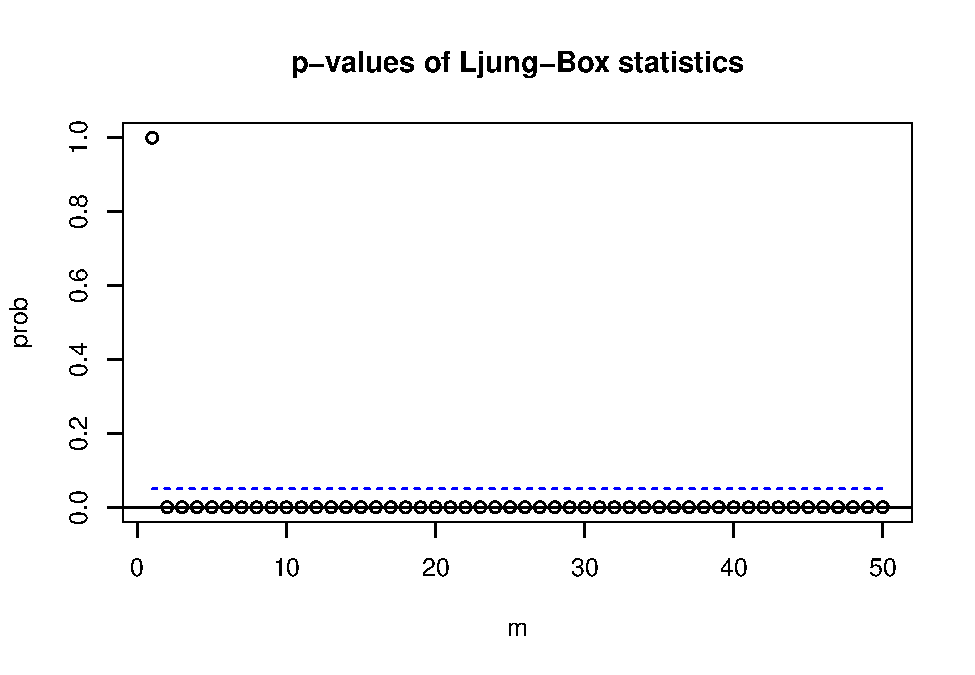
\includegraphics{solution_exercise_5_files/figure-latex/unnamed-chunk-23-1.pdf}

\begin{Shaded}
\begin{Highlighting}[]
\KeywordTok{VARorder}\NormalTok{(}\DataTypeTok{x =}\NormalTok{ fx_var1.fit}\OperatorTok{$}\NormalTok{residuals}\OperatorTok{^}\DecValTok{2}\NormalTok{, }\DataTypeTok{maxp =} \DecValTok{20}\NormalTok{)}
\end{Highlighting}
\end{Shaded}

\begin{verbatim}
## selected order: aic =  20 
## selected order: bic =  13 
## selected order: hq =  13 
## Summary table:  
##        p      AIC      BIC       HQ     M(p) p-value
##  [1,]  0 -37.4176 -37.4176 -37.4176   0.0000  0.0000
##  [2,]  1 -37.4290 -37.4238 -37.4272  64.6885  0.0000
##  [3,]  2 -37.4592 -37.4488 -37.4556 158.9360  0.0000
##  [4,]  3 -37.4619 -37.4463 -37.4564  21.3438  0.0003
##  [5,]  4 -37.4713 -37.4505 -37.4640  54.6839  0.0000
##  [6,]  5 -37.4750 -37.4490 -37.4659  26.6857  0.0000
##  [7,]  6 -37.4840 -37.4528 -37.4730  52.5478  0.0000
##  [8,]  7 -37.4891 -37.4527 -37.4764  33.6938  0.0000
##  [9,]  8 -37.4923 -37.4507 -37.4777  23.6494  0.0001
## [10,]  9 -37.5008 -37.4540 -37.4844  50.4637  0.0000
## [11,] 10 -37.5012 -37.4492 -37.4830   9.8909  0.0423
## [12,] 11 -37.5119 -37.4548 -37.4919  61.2238  0.0000
## [13,] 12 -37.5143 -37.4519 -37.4925  19.8154  0.0005
## [14,] 13 -37.5278 -37.4602 -37.5041  75.0385  0.0000
## [15,] 14 -37.5287 -37.4559 -37.5032  12.2053  0.0159
## [16,] 15 -37.5307 -37.4527 -37.5034  17.9167  0.0013
## [17,] 16 -37.5310 -37.4479 -37.5019   9.7336  0.0452
## [18,] 17 -37.5322 -37.4438 -37.5012  13.4969  0.0091
## [19,] 18 -37.5317 -37.4381 -37.4989   5.3946  0.2491
## [20,] 19 -37.5325 -37.4338 -37.4979  12.0269  0.0172
## [21,] 20 -37.5391 -37.4352 -37.5027  40.5684  0.0000
\end{verbatim}

\begin{Shaded}
\begin{Highlighting}[]
\KeywordTok{plot.ts}\NormalTok{(fx_var1.fit}\OperatorTok{$}\NormalTok{residuals}\OperatorTok{^}\DecValTok{2}\NormalTok{)}
\end{Highlighting}
\end{Shaded}

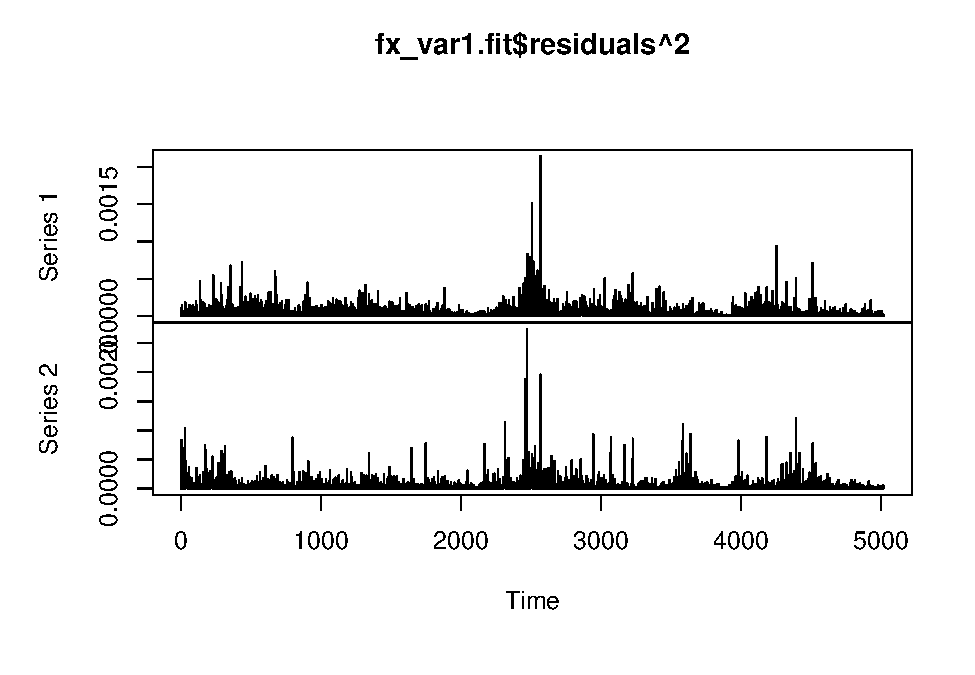
\includegraphics{solution_exercise_5_files/figure-latex/unnamed-chunk-23-2.pdf}

Plenty of lagged cross-/auto correlations. Information criteria suggest
high lag orders. Fitting a \(\VAR\) appears sensible.

\begin{itemize}
  \item[f.)] Can you rule out weak stationarity for the growth rates of the exchange rates only based on your findings up to this point?
\end{itemize}

No.~Weak stationarity is about time-invariance regarding the
\emph{unconditional} expecation and variance. Heteroscedasticity can be
a violation of weak stationarity, simply because the variance is not
constant over time. But if we are able to sufficiently model the
variation of the variance using a VAR, we are in fact facing
\emph{conditional} heteroscedasticity:
\(E(a_{t}^2) = \sigma_{t} * \epsilon_{t}\) with \(\epsilon_{t}\) as
white noise. And as we learned before, a stable VAR with white
noise-innovations yields a stationary time series. This is analogous to
a stationary VAR, where the conditional expectation of the observations
may differ from the unconditional expectation (depending on past
observations).

\end{document}
